\documentclass{acm_proc_article-sp}

\usepackage{color}
\usepackage{algorithm}
\usepackage{algorithmic}
\usepackage{url}

\begin{document}

\title{MalwareVis: Entity-based Visualization of Malware Network Traces}
%\title{MalwareVis: Cell-based Visualization of Malware Network Traces}

\numberofauthors{1}
%\author{}
%\author{Submit to VizSec 2012 for blind review}
% need to confirm if the professors are willingly to let their names appear
\author{Wei Zhuo \qquad Yacin Nadjin \\
\affaddr{Graphics, Visualization and Usability Center} \\
\affaddr{Colleage of Computing}\\
\affaddr{Georgia Institute of Technology}\\
\email{wzhuo3, yacin@cc.gatech.edu}
}


\maketitle



\begin{abstract}
This paper presents MalwareVis, a utility that provides security researchers a method to browse, filter, view and compare malware network traces as entities.

Specifically, we propose a cell-like visualization model to view the network traces of a malware sample's execution. This model is a intuitive representation of the heterogeneous attributes (protocol, host ip, transmission size, packet number, duration) of a list of network streams associated with a malware instance. We encode these features into colors and basic geometric properties of common shapes. The list of streams is organized circularly in a clock-wise fashion to form an entity. Our design takes into account of the sparse and skew nature of these attributes' distributions and proposes mapping and layout strategies to allow a clear global view of a malware sample's behaviors. 

We demonstrate MalwareVis on a real-world corpus of malware samples and display their individual activity patterns. We show that it is a simple to use utility that provides intriguing visual representations that facilitate user interaction to perform security analysis.    


 
\end{abstract}



\category{H.5}{Information Interfaces and Presentation}{User Interfaces}
\category{C.2.0}{Computer-Communication Networks}{General}[Security and Protection]
\category{I.3.8}{Computer Graphics}{Applications}
\terms{Visualization, Security}
\keywords{Malware Analysis, Network Behavior Visualization}



\section{Introduction}
\label{sec:Introduction}
\begin{figure*}
	\centering
		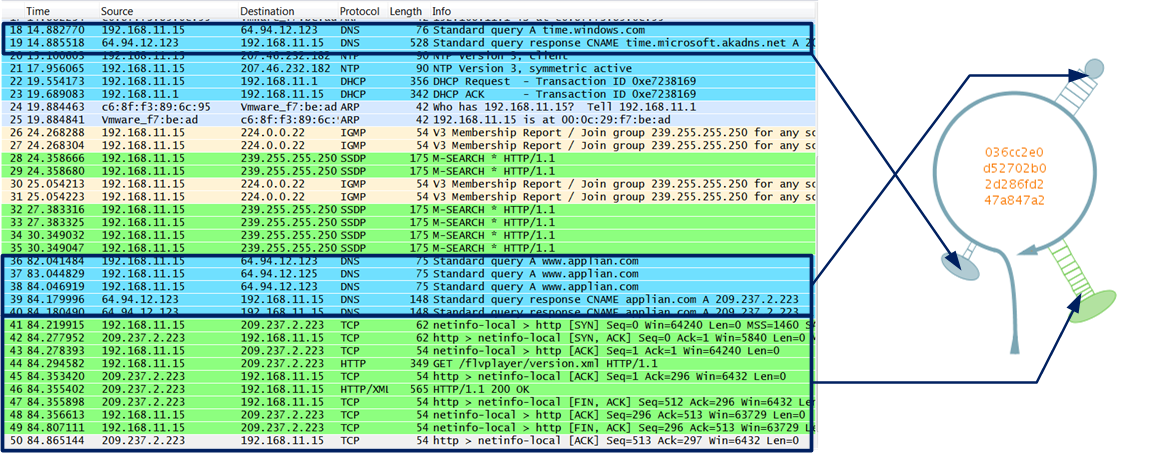
\includegraphics[width=0.78\linewidth]{pics/Mapping.png}
	\label{fig:Mapping}
        \caption{We illustrate our mapping scheme with a simple network packet
        traces generated by malware~(036cc2e0): there are three
        streams of packets~(as highlighted by rectangles in the flow records
        produced by Wireshark~\cite{Wireshark}) are mapped to three cilia in
        the cell view on the right. The user can select a cilium for detailed
        information about the stream.}
\end{figure*}


Malware remains at the forefront of most security threats on the Internet. Nearly every existing malware instance relies on network communication to facilitate its attacks, such as communicating with its command and control (C\&C) server, sending spam emails or operating in a fast-flux service network. Therefore, network traces are commonly used to characterize a malware sample's behavior. As an essential technology that combats illegal income for the attackers, malware analysis has been playing a crucial role in supplying signatures for detection systems.

There is a growing need for visual presentations in the workplace of malware analysis: new instances of ``in the wild'' malware samples are collected daily. In a typical analysis scenario, each malware instance is run in a controlled environment where its host-level and network-level activities are captured as host and network traces. In order to keep track of each sample, security researchers maintain large databases of network traces. Due to their sheer size, it is a daunting task to look into the details of each sample.

Current malware analysis approaches pose several challenges to the analytic
process itself which complicate visualization design. First, network traces
often contain network information that is not relevant to the actual malicious
behavior. For example, network traffic generated by the operating system.
Having to visualize everything not only complicates the design, but also causes
confusion to the analysts. Malware samples seen in the wild tend to use only a
couple of protocols, such as DNS and TCP, to perform their malicious behavior.
To reduce clutter, we do not visualize less common protocols by default.
Second, the analyst can easily lose the big picture of malware activities by
focusing on individual packets. To handle this, we aggregate packets into
streams separated by protocol. Specifically, we focus on DNS and TCP streams as
they are often used by malware for communication. Third, streams can vary
drastically in packet size and these uneven distributions present themselves in
nearly every attribute space (e.g. total size of transmission, starting time,
duration). Linearly mapping these attributes not only consumes screen
real-estate, but also draws the viewer's attention away from those small but
potentially important streams. Lastly, showing all relevant attributes in a
single, clear view requires an original design. In the absence of an intuitive
presentation of sets of network traces, malware behavior analysis will remain
tedious.

The goal of this paper is to present a visualization system and a model design
that address the above challenges. Our work claims the following contributions:
\begin{itemize}

	\item \textbf{Data collection and preprocessing.} The malware network traces were captured by packet sniffer software in a controlled environment. The preprocessing consists of two steps: \emph{pruning} and \emph{bundling}. The raw network data are pruned by preserving protocols known to be used commonly by malware seen in the wild be default. Other protocols can be viewed if an analyst wishes to do so. Then we bundle the packets according to their protocols and hosts so that each stream of communication is semantically clear.

	\item \textbf{Interface and visualization metaphor.} We design an intuitive view, the \emph{cell view}, to represent a set of streams generated by any malware instance. A cell view consists of a \emph{circular timeline}, a \emph{disk panel} to display details-on-demand, and a set of \emph{cilia} oriented clockwise along the timeline to represent the set of streams. This metaphorical structure allows the viewer to select and compare among streams as well as between malware instances.

	\item \textbf{Mapping and layout techniques for sparsely distributed attributes.} As explained earlier, the majority of the communication~(in terms of the number of packets, transmission size) takes place within a small percentage of streams. Also, many streams may occur within a short period of time. To cope with these uneven distributions, we use geometric sequences and inverse logarithms to map discrete or continuous attribute values. We also present a recursive angle mapping algorithm that helps produce equalized layout for viewing streams that are cluttered over time.
\end{itemize}

This paper is organized as follows. Section~\ref{sec:prior} introduces several related security visualization systems. Section~\ref{sec:overview} presents an expository account of malware analysis infrastructure for the benefit of readers who are not familiar with the technique. We then introduce our design and implementation in Section\ref{sec:implementation}. We apply the visualization model to a corpus of real-world malware samples and Section~\ref{sec:interaction} introduces user interaction scenarios with different components of MalwareVis. Finally, Section~\ref{sec:discuss} discusses and reflects on the project process; Section~\ref{sec:conclude} concludes the paper.







\section{Prior Art}
\label{sec:prior}
Most of the related network visualization systems so far has been traffic-centric with explicit focuses on each record of flows. For example, the work of McPherson and Ma~\cite{McPherson:2004} presents PortVis, which visualize a large network flow data collected at certain Internet gateway. Their system allows interactive timeline filtering and histogram summarization on port activities. NVisionIP~\cite{Lakkaraju:2004}, introduced by Lakkaraju and his colleagues, focuses on the static visual representation of the IP network traffic in a 2D scatter plot named galaxy view. The other two views~(the small multiple view and the machine view) complement the main view by providing bar charts of various flow counts. TNV by Goodall et al.~\cite{Goodall:2005} aims to visualize the source, destination and the time attributes in a single view. To allow the user to explore the area of interest in greater detail, TNV can zoom in on traffic through bifocal display techniques. Rumint~\cite{Conti} is another full-fledged, time-oriented network traffic analyzer that captures live traffic and supports playing back the traffic. 

Apart from scatter plots and histograms/bar-charts, linked graphs have become popular representations of network flows. Based on force-directed graph layout techniques, Afterglow~\cite{Marty} is a collection of utilities for generalized communication network visualization. Recently, Blue and his colleagues present NetGrok~\cite{Blue:2008} that consists of graph and treemap views. In their graph view, the IP layer communications with the local host are visualized as a star network with other hosts organized around based on their IP addresses. 
Although using graphs for security visualization has increased in popularity,
it is unclear to the authors how to incorporate the time-series nature of network 
flow data into graphs without using a complementary view.

Compare to previous traffic-centric visualization systems, the major innovation and advantage of MalwareVis lies in its entity-based design. The idea is to visualize the network traces associated with each malware instance as a whole. It is natural to represent the overall flow associated with each sample as one model for the purpose of identifying potentially interesting patterns. 

For example, Quist and Liebrock visualize the compiled executables from monitoring malicious program execution~\cite{Quist11}. While our work focus on malware network traces, the purpose is similar---to allow the analysts to identity particular patterns of network traffic. Based on this idea, we design a intuitive visualization model, the cell view, to present behaviors of malware network communications.       


\section{System Overview}
\label{sec:overview}
\begin{figure}
	\centering
		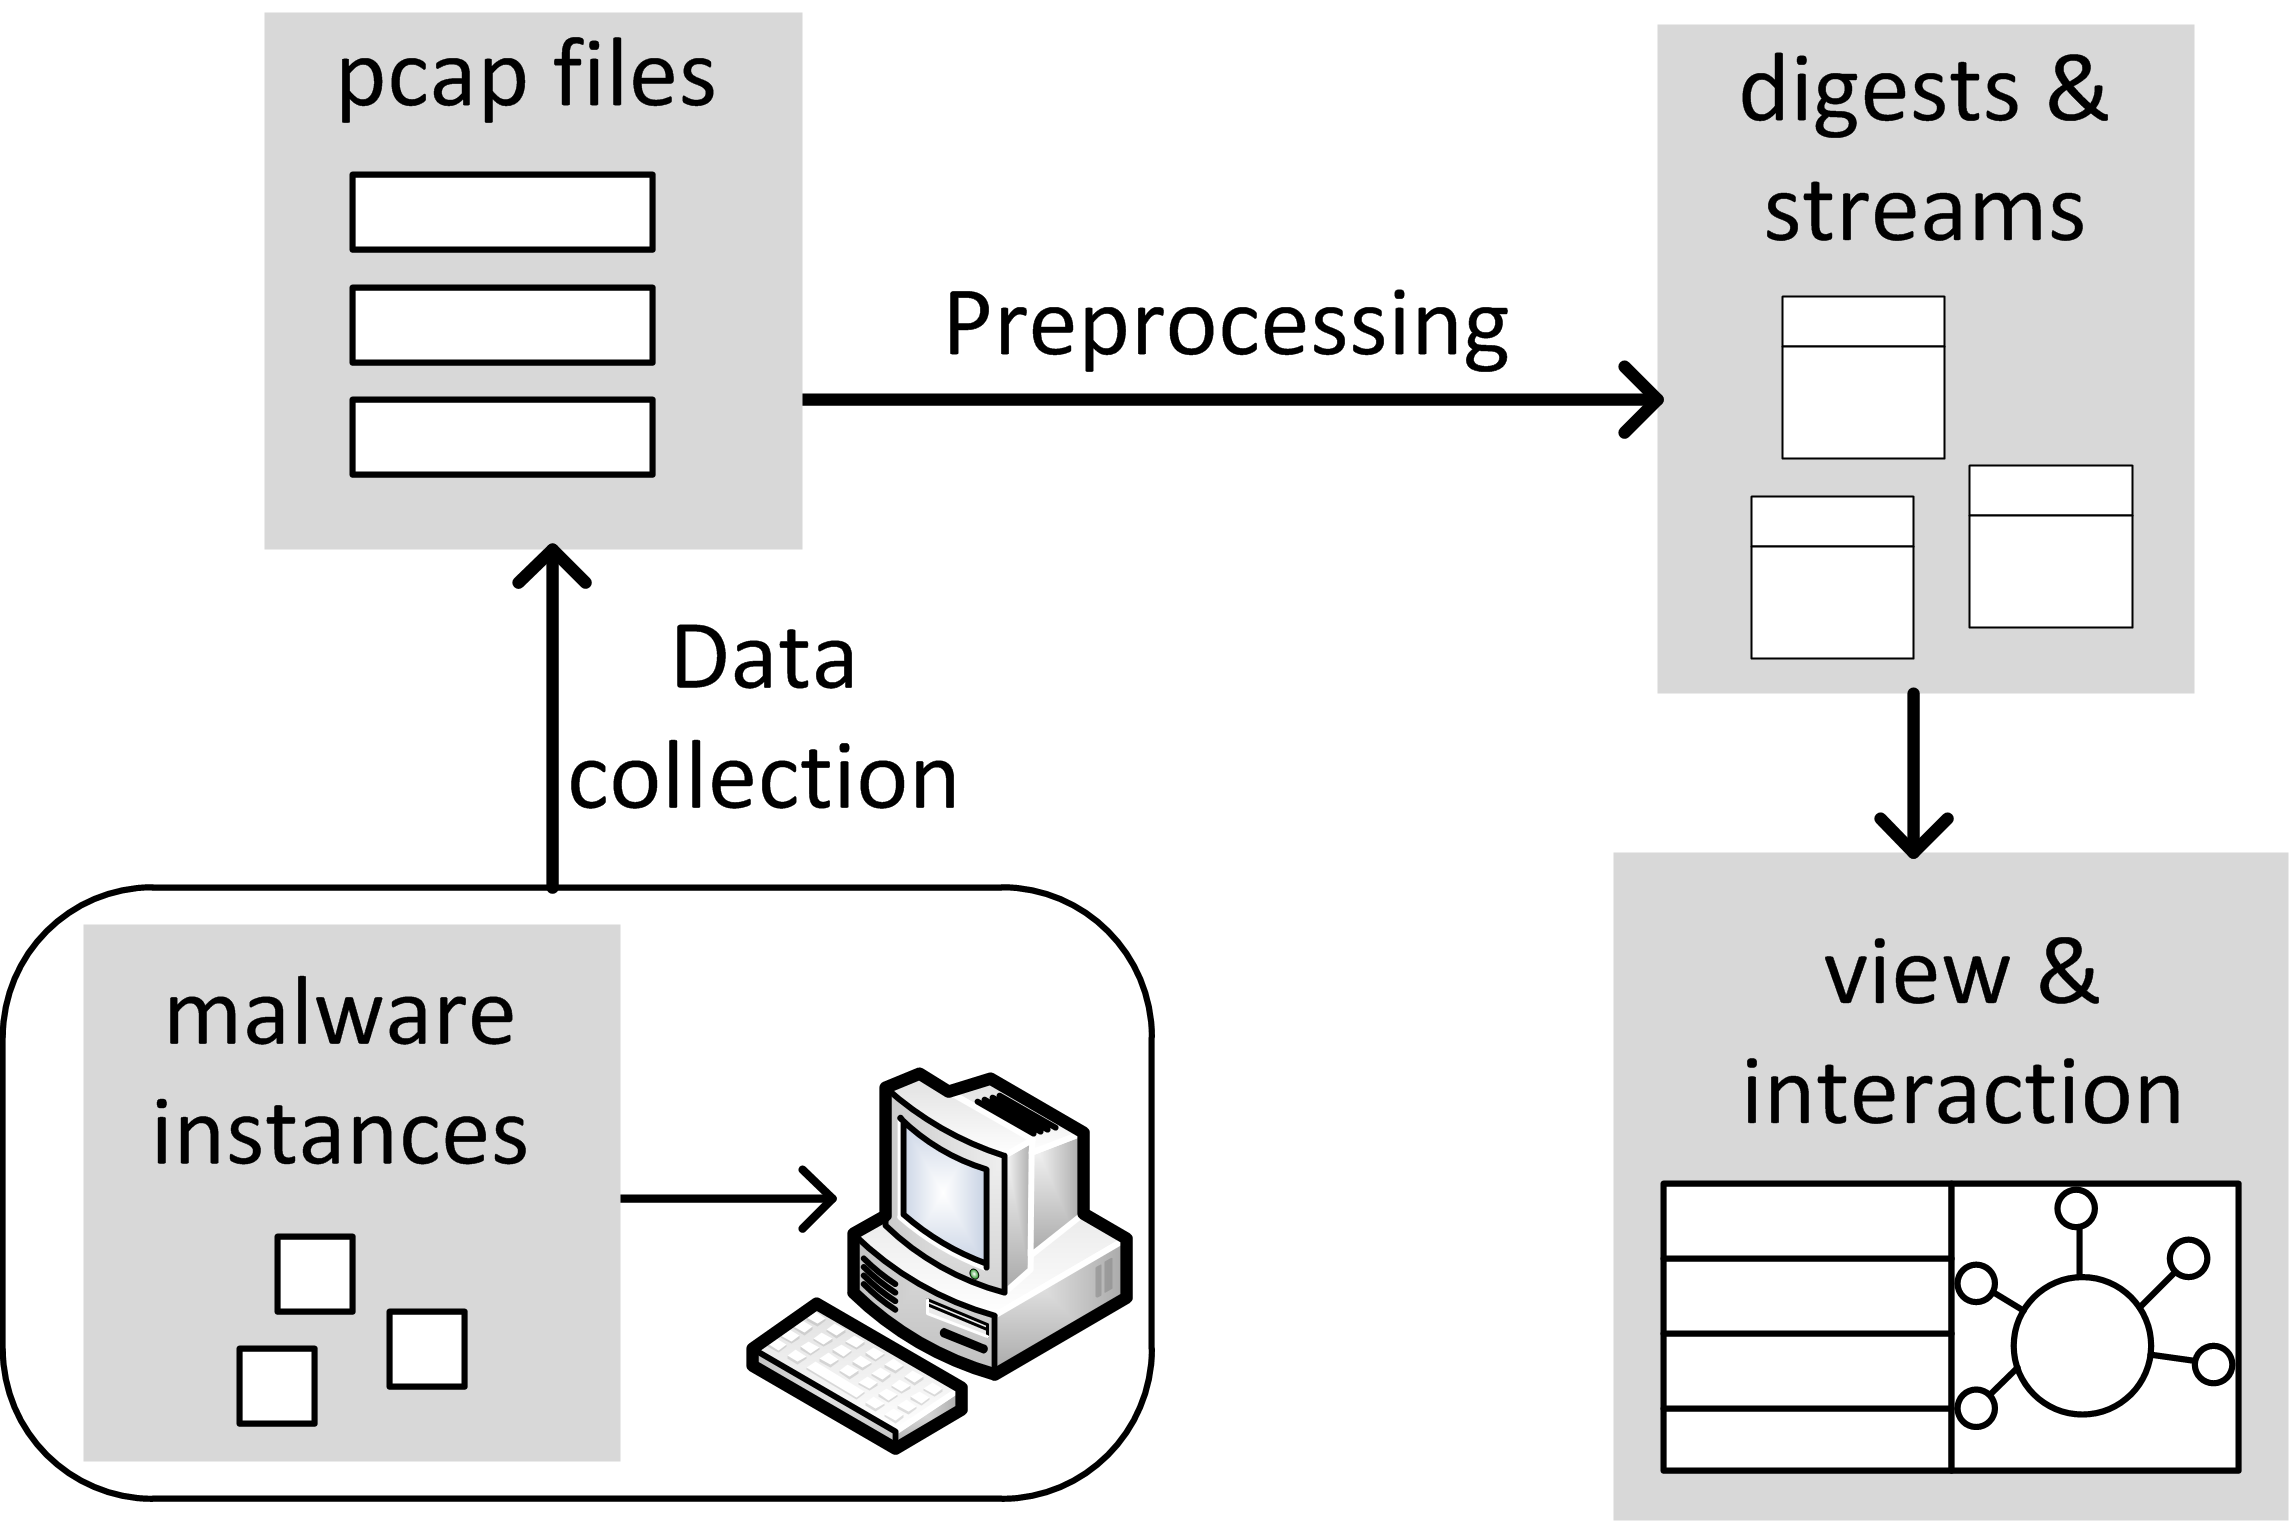
\includegraphics[width=\linewidth]{pics/Overview.png}
	\caption{The overview of our malware visual analytic system. The user-end view and interaction rely on three primary modules: data collection, preprocessing and visualization.}
		\label{fig:Overview}
\end{figure}

We show an overview of our malware visual analytic system in
Figure~\ref{fig:Overview}, and discuss how malware network data are captured,
processed and visualized in this section. This process consists of three
primary steps: \emph{data collection}, \emph{preprocessing}, and
\emph{visualization}.

\textbf{Data sources.} First, we gather a corpus of malware samples to use for
evaluation purposes. 200 MD5 unique malware samples were randomly selected from
malware collected during April 2011. We use multiple sources that provide
approximately 6,000 MD5 distinct samples per day taken from low interaction
honeypots, web crawlers, spam email filters, and user submissions. We restrict
our test set to only malware samples that exhibit network behavior during
execution. We analyze the malicious binaries by executing them for three minutes
in a virtualized dynamic malware analysis system that runs malware samples in
kvm~\cite{kvm} and records all the network traffic into packet traces as pcap
files\footnote{\url{http://www.tcpdump.org}}. Our visualization system is not
dependent on any particular dynamic analysis system and similar systems
described in the literature could serve as drop-in
replacements~(\cite{Bayer06}~\cite{Dinaburg08}),
Precautions were taken to prevent the executing malware from acting
maliciously; specifically, we redirect SMTP traffic to a spam trap, blocked
connections to ports commonly used by exploits and blocked traffic to other
local machines.

\textbf{Preprocessing.} Next, we parse pcap files into a set of appropriately
formatted documents which we refer to as malware entities. Each entity is of
the form

\verb+<Digest D | ArrayList<Stream> S>+

The structure \emph{Digest} consists of a sample's MD5, the total number of
packets, the total size of transmission, the total number of streams, and the
packet trace's duration. The list of streams are extracted from the protocol
information in the pcap file. Specifically, each stream includes attributes
such as host~(IP or domain name), protocol~(DNS or TCP), number of
packets~($n$), size of transmission~($z$), offset from the initial start
time~($s$), duration~($t$), and whether the stream ended successfully or not. A
DNS stream is defined as a DNS request and its corresponding response and a TCP
stream begins with a 3-way TCP handshake and concludes with successful or
unsuccessful termination.

\textbf{Visualization.} The visualization module generates table views and cell
views. Given a set of parsed and preprocessing entities, the user browses the
table of digests and selects one or more targets for analysis. Then, the
application generates a stream table and a cell view for each selected entity.
Our attributes mapping and layout algorithms run in real-time for most of the
malware entities supplied. In a typical visual analysis scenario, the user
interacts with the cell view by selecting a `cilium' that represents a stream of
interest. Details of the stream, such as its host IP and country code, are
displayed at the disk panel located at the center of the cell view. The user
can adjust the layout parameters for the circular timeline interactively so as
to improve the clarity of the set of cilia~(Sec.~\ref{sec:timeline}).



\begin{figure*}
	\begin{center}
	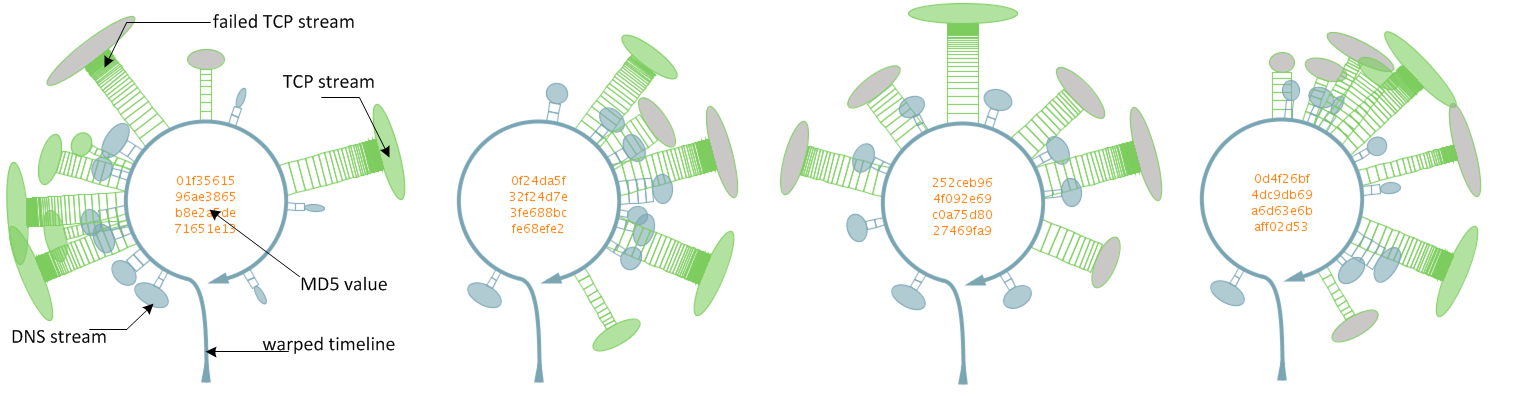
\includegraphics[width = 0.98\linewidth]{pics/Samples.png}
	\label{fig:samples}
	\end{center}
	\caption{We show the cell views generated by MalewareVis for 4 maleware instances. From left to right, the views each represent 5661, 313, 3527, 1043 records in their corresponding pcap files. We annotate on the first view~(the detailed mapping scheme is explained in Sec.~\ref{sec:implementation}); the second view and the fourth view show similar behaviors in terms of communication patterns. Different behaviors associated with different samples are intuitive to see.}
\end{figure*}

\section{Cell View Implementation}
\label{sec:implementation}

This section presents our design of the cell view. We first introduce different components of a cell view and their implementations in Sec.~\ref{sec:components}. Then we present in Sec.~\ref{sec:mapping} the detailed mapping schemes that encode the various attributes to properties of simple geometric shapes. In Sec.~\ref{sec:timeline} we present a layout algorithm inspired from fast tone-mapping technique to avoid cluttered drawing on the timeline.  

\subsection{Components}
\label{sec:components}
A cell view has three basic components: a timeline, a disk panel and a set of cilia.  

\textbf{Timeline.} As shown in Fig.~\ref{fig:timeline}, the time line is an directional open curve joined by an circular arc and a quadratic Bezier curve. The arc is of radius $R$, centered on screen and spanning an angle from $\delta$ to $2\pi-\delta$, where $\delta$ is set to a small positive value ($\frac{\pi}{12}$ in our work) to differentiate the starting point from the end point. The control points of the Bezier curve are specified by $\delta$ and $R$ in order to let the curve joins the arc with tangent continuity.

\begin{figure}[h!]
	\centering
		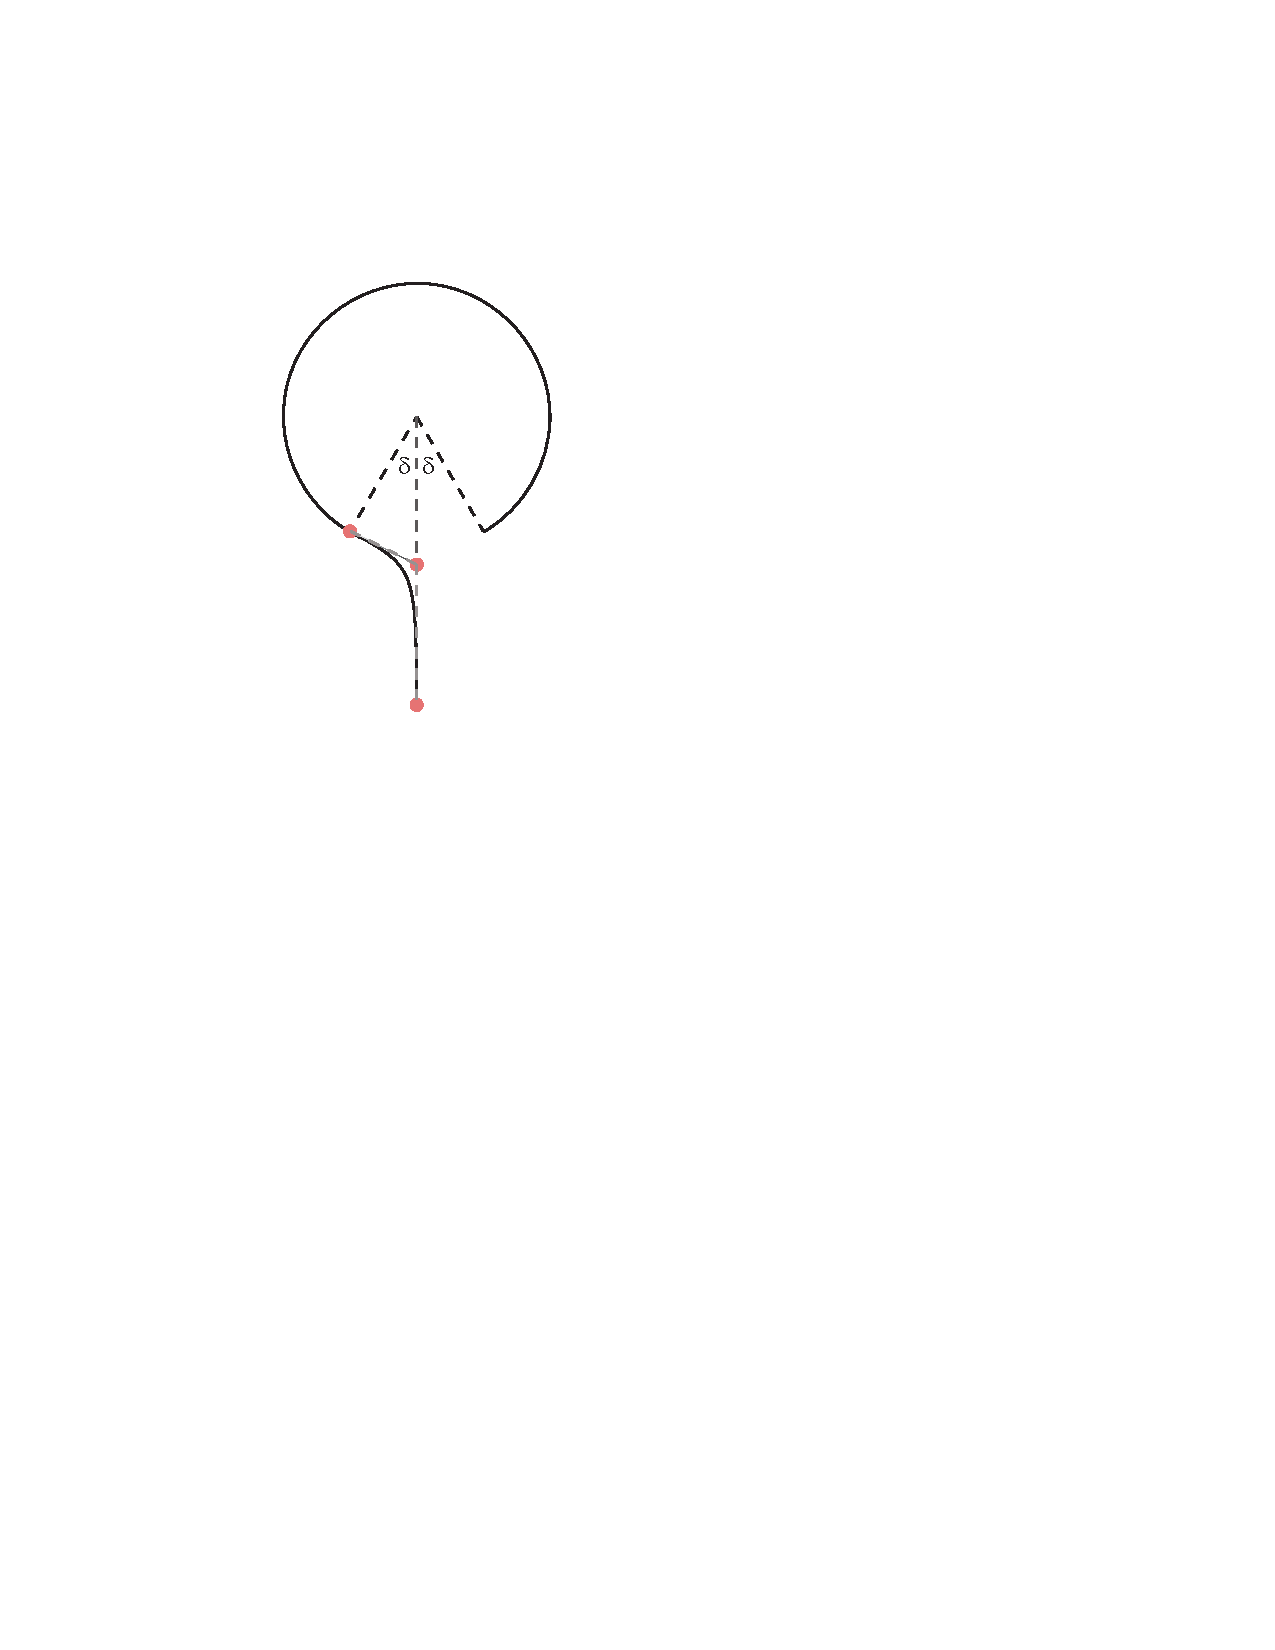
\includegraphics[width=1.3in]{pics/timeline.pdf}
	\label{fig:timeline}
	\caption{The timeline is an open curve joined by an arc and a quadratic Bezier curve: the red dots are the control points of the Bezier curve.}
\end{figure}

The use of circular timeline is not new~(e.g.~\cite{Chuah:1998}) and is commonly appeared as a model in geology and news data visualization for presenting events that are evolving or periodic in nature. Here the motivation is to view malware network traces as an entity. We believe that using a circular timeline instead of a straight timeline better promotes this impression.

\textbf{Disk Panel.} The circular timeline delimits a round area which is used to display the primary key of the malware instance or details of a user-selected stream. In the viewing mode, the unique MD5 value is shown on the disk panel. In the interaction mode, the disk panel display attribute values of the user-selected stream. It is possible to show the details of a stream near the cilium representing this stream, or in another pop-up panel; nevertheless, using the disk panel is a more economical choice in terms of minimizing the total screen space necessary for the view. 

\textbf{Cilium.} Each cilium represents a stream of network communications. A cilium has a \emph{stem} and a \emph{head}. The stem of the cilium is a quad strip. Each quad represent a packet and hence the longer the stem the larger is the number of packets being transmitted. The width of the stem is correlated with the duration of the stream. The head of the cilium is a ellipse whose width encodes the size of transmission. Note that in a real-world scenario, the number of packets, duration and size are highly correlated with each other. Hence, the width of a cilium's head commonly scales with the length of its stem. Outliers, such as a 'short' cilium with a 'wide' head or a 'tall' cilium with a 'slender' stem , might be indicative of interesting behavior.     

\textbf{Drawing.} All geometric dimensions~(timeline radius, cilium height, width, etc.) are relative to the screen size, hence the cell view can scale without loss of quality. Each cilium object is associated with a drawing function~(\verb+drawCilium()+) that display the cilium with transparency in the local coordinate system. The transformation matrix stack is used to draw a cilium in the global coordinate system:
\begin{verbatim} 
pushMatrix(); 
translate(P.x, P.y); 
rotate(a); 
drawCilium(); 
popMatrix();
\end{verbatim}
where $P$ is the contact point of the cilium on the timeline determined the plan angle $a$ and the timeline's center $O$ and radius $R$.  

\subsection{Attribute Mapping}
\label{sec:mapping}
As expressed earlier, we use nonlinear mapping functions to transfer attribute values to geometric properties since linear mapping may require unbounded area. The design guideline of each mapping function is to limit each geometric dimension to be within a lower bound and a upper bound and is a monotonically increasing function of the input attribute value.   

\textbf{Mapping number of packets~$n$ to cilium stem height~$h$:} The stem of the cilium is a quad strip where each quad denotes a packet. The cilium height $h$ is the sum of the set of quad heights $\{h_i\}$, which forms a geometric sequence with $r$ as the scale factor:
\[ r = \frac{h_{max} - h_{min}}{ h_{max}} \]
For example, if a stream has $n$ packets, the height of its stem is
\begin{equation}
h = h(n) = \sum_{i=1}^n h_i = h_{max}(1-r^n)
\end{equation}
Hence, $h$ is bounded by $h_{min}$ and $h_{max}$, and $h(n)$ is monotonically increasing in $n$. 

\textbf{Mapping duration~$t$ to cilium stem width~$w$:} The width $w$ of the stem is mapped from the duration $t$ of the stream by the following transfer function
\begin{equation}
w = w(t) = w_{max} -  \frac{w_{max} - w_{min}}{t+1}
\end{equation}
This would limit the width of the stem to $w_{max}$ and $w(t)$ is a increasing function of $t$. 

\textbf{Mapping size of transmission~$z$ to cilium head width~$w$:} Similarly, the width $l$ of the oval head of the stem is computed from the size of the stream, denoted by $z$:
\begin{equation}
l = l(z) = l_{max} - \frac{l_{max} - l_{min}}{log(z)}
\end{equation}
As the sizes of transmission of different streams can be drastically different~(ranges from $10^2$ to $10^6$ bytes), we use logarithm of $z$ in the mapping function. 

\subsection{Layout on Timeline}
\label{sec:timeline}
To strengthen the visualization as a cell entity, we clock-wisely oriented the set of streams around the circular timeline. Each stream has a starting time which we denote as $s_i$, and the position it appears on the circular timeline is determined by its contacting angle $a_i$. The relative order and the intermissions of a set of streams are important characteristics of a malware instance's behavior.  
     
Therefore, given a set of starting times $\{s_i\}, i=1,...,k$, we want to compute a set of angles $\{a_i\}$ bounded by the mappable range $[ \delta, 2\pi-\delta]$. Assume that $\{s_i\}$ is sorted. $s_1$ is the smallest and mapped to $\delta$ and $s_k$ is the largest and mapped to $2\pi-\delta$. As mentioned earlier, the distribution of $\{s_i\}$ is very uneven because multiple streams of communications may occur in a very short time period. Hence, linearly mapping $\{s_i\}$ to the mappable range may lead to overlappings and visual clutter, as shown in Fig.~\ref{fig:Tune}~left. In order to improve clarity while preserving the relative order as they appear in $\{s_i\}$, we present a recursive range mapping algorithm in Alg.~\ref{alg:mapping}. This algorithm is inspired by fast tone reproduction techniques for visualizing high dynamic range image data~\cite{Duan:2004} based on the fact that the distribution of HDR data tends to be sparse. Here, the set of starting times $\{s_i\}$ is analogous to the raw HDR image data and the mappable range~($[ \delta, 2\pi-\delta]$) is analogous to the viewable intensity range~($[0, 255]$) in the tone-mapped image. The idea of fast tone-mapping is to scale the mapping range according to the input data histogram: the time period that contains more incidences of streams is mapped to a larger range. 
  
\textbf{Algorithm Tuning.} Specifically, $\alpha \in [0, 1]$ is the parameter that specifies the scaling effect: the larger $\alpha$ is, the more equalized the mapping is. If $\alpha=0$, Alg.~\ref{alg:mapping} is essentially a linear mapping, which causes visual clutter due to that multiple streams typically start together. If $\alpha = 1$, Alg.~\ref{alg:mapping} is the equalized mapping where the streams appear uniformly spaced. However, the equalized mapping does not show intermissions, such as a long period of inactivity after the first DNS stream in Fig.~\ref{fig:Tune}~right.       

\begin{algorithm}
\floatname{algorithm}{Alg.}
\renewcommand{\algorithmicrequire}{\textbf{Input:}}
\renewcommand{\algorithmicensure}{\textbf{Result:}}
\caption{Recursive range mapping: $map(i, j, a_{min}, a_{max})$ }
\label{alg:mapping}
\begin{algorithmic}
\REQUIRE subarray indices $i,j$ of input array $s$, \\
         mapping range $[a_{min}, a_{max}]$ 
\ENSURE set angles in output array $a$
\STATE $a_{mean} \Leftarrow \frac{a_{min} + a_{max}}{2}$
\IF{$i \geq j$}
    \STATE $a_i \Leftarrow a_{mean}$
    \STATE return
\ENDIF
\STATE $s_{mean} \Leftarrow \frac{s_i+s_j}{2}$, 
\STATE $s_{median} \Leftarrow s_{(i+j)/2}$  
\STATE $cut \Leftarrow \alpha s_{median} + (1-\alpha)s_{mean}$
\STATE $ci\Leftarrow$ index of $cut$ in array $s$
\IF{$ci==i$}
	\STATE $a_i \Leftarrow a_{min}$
	\STATE $map(ci+1, j, a_{mean}, a_{max})$
	\STATE return
\ENDIF
\IF{$ci==j$}
	\STATE $a_j \Leftarrow a_{max}$
	\STATE $map(i, ci-1, a_{min}, a_{mean})$
	\STATE return
\ENDIF
\STATE $map(i, ci-1, a_{min}, a_{mean})$
\STATE $map(ci, j, a_{mean}, a_{max})$
\end{algorithmic}
\end{algorithm}


\begin{figure*}
	\centering
		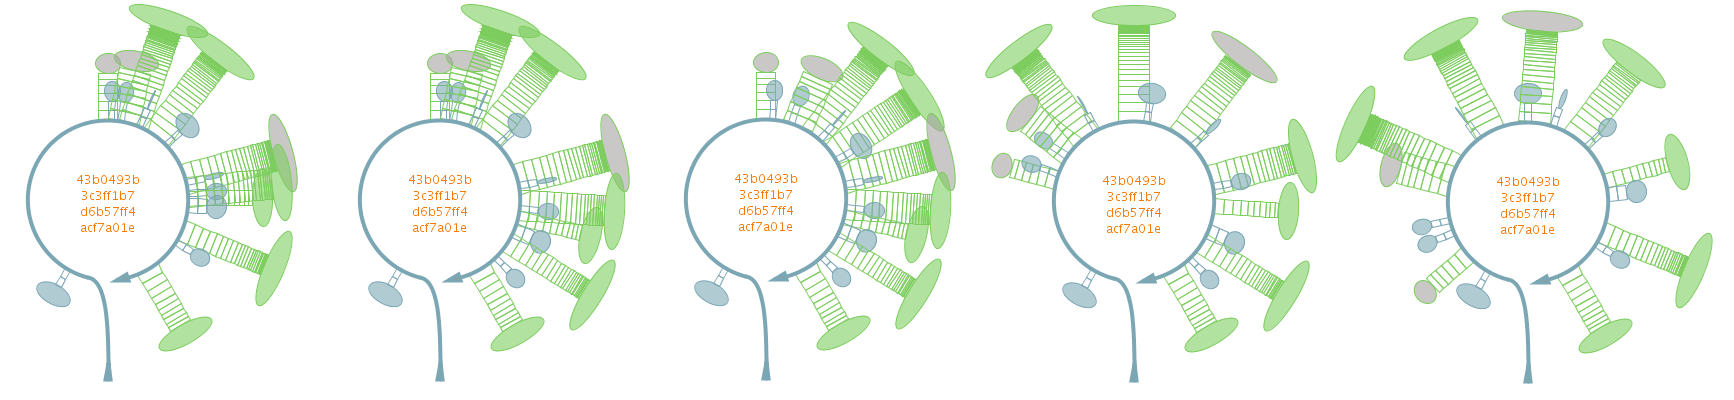
\includegraphics[width = 0.98\linewidth]{pics/Tune.png}
	\label{fig:Tune}
	\caption{From left to right, we show a sequence of visualizations of the same malware instance with increasing $\alpha$ values: (a) linearly mapping the starting times to angles would results in visual clutter; (d) equalized mapping helps to reduce the overlapping effects.}
\end{figure*}





\section{User Interaction}
\label{sec:interaction}
In this section, we present the user interface of MalwareVis. 
\begin{figure*}
	\centering
		\includegraphics[width = 0.88\linewidth]{pics/Screen.png}
	\label{fig:Screen}
	\caption{MalwareVis's user interface has a table view that allows the user to browse and filter malware entities and the cell view for graphical representations, interaction and comparision.}
\end{figure*}

To start, the user can select a set of pcap files (typically a corpus of malware network traces) and MalwareVis parses them into a collection of entities~(Fig.~\ref{fig:Overview}). Parsing and preprocessing takes approximately 30 seconds for 95 pcap files~(average file size 722KB). In addition to reading raw pcap files, the user can select a set of previously saved entities for quickly initiating the application. 

\textbf{Table View: } As shown in Fig.~\ref{fig:Screen}, the program then generates table views. The \emph{pcap table} displays the entity digests, each of which is a summary of a list of communication sessions recorded by a pcap file. The user can browse the list of entities and search or filter them based on MD5 values and duration. The lower part of the table view is the \emph{stream table} that list a set of streams of a user-selected entity. 

\textbf{Single Cell View:} After the user select a entity, she can create a cell view of the entity by clicking the ``single'' button in the cell view control panel. A cell view appears in a very small fraction of a second. In the cell view, the user can interact with a string of cilia: the user can select a cilium by clicking the oval head of the cilium. Then the disk panel shows the detailed stream information represented by this cilium. It also queries a GeoIP database to identify the country name and flag of the host IP if it is a routable IP address. The user can also select from the stream table and its corresponding stream and cilium are highlighted in both views. 

\textbf{Timeline:} The user can change the value of $\alpha$ in the timeline mapping algorithm~(Alg.~\ref{alg:mapping}) from the slider in the cell view control panel. Notice that when sliding, the cell view redraws the set of cilia at each frame. This creates intermediate frames between the two views of different $\alpha$ values~(Fig.~\ref{fig:Tune}). Therefore, the user can view the layout equalization processing on the timeline as a animation.   

\textbf{Multiple Cell Views:} The user can also select multiple malware entities. Then, stacked cell views of a list of the selected entities can be created by clicking the ``multiple'' button in the cell view control panel. The user can compare the visual representations of multiple malware samples~(Fig.~\ref{fig:samples}) and interact with each view as one would interact with a single cell view. 

 

\section{Reflection and Discussion}
\label{sec:discuss}
This section discusses the project collaboration process, the feedbacks and ideas for potential future work.

\textbf{Collaboration.} This project has involved close collaboration between students at the graphics$\&$visualization and the information security centers. Initially, the visualization design and the data collection processes were conducted separately. However, to build a visualization model that addresses both utility and aesthetic concerns requires close collaboration among participants. Hence in the development phase, participants met and discussed issues with data processing, visualization and user interaction on a regular basis. Convenient design and collaboration was made possible through shared repository of open source interfacing tools~(\cite{jython}~\cite{dpkt}) and the Processing visualization library~\cite{Processing}. 

\textbf{Feedbacks.} We found building MalwareVis to be a rewarding experience: not only the participants with different backgrounds have learned from each other, but the users are intrigued by our design as well during informal user testing. From their feedbacks, we have concluded two major advantages of the cell view. The first advantage is that it provides a global view: a single cell view is able to represent up to 6000 flow records in a pcap file without significant visual clutter~(Fig.~\ref{fig:samples}). The second advantage is that it provides a graphical user interface that allows the user to analyze different malware behaviors interactively.

\textbf{Future Development.} During our informal user testing, a user asked if there is any relationship between different malware instances and how to visualize them. Binary and n-ary relationships do exist within a corpus of malware instances. For example, malware frequently found in honeypots actually behave as downloaders and simply download, install and execute other malicious binaries. Furthermore, malware is often packed resulting in binaries that are MD5 unique, but exhibit identical behavior. Currently, MalwareVis does not support highlighting these relationships automatically, but we believe this is a possible direction for future work. 
 





\section{Conclusion}
\label{sec:conclude}

Malware network traces are important characteristics of a malware sample's behavior. To address the need of a visual representation in the workplace of malware analysis, we have develop a processing and visualization tool, MalwareVis, that allow a security analyst to filter, select, visualize, and compare malware network traces. It reads pcap files, processes them into streams and generates cell views for the user-selected malware entities interactively. In this paper, we have described our visualization design and demonstrate the advantages of using cell views. In the future, we will explore several areas such as visualizing the relationship among a collection of malware network traces.     

\section{Acknowledgements}
We would like to thank reviewers for their comments, Prof. Jarek Rossignac, Prof. Wenke Lee, Dr. Wes Bethel and Prabhat for their suggestions, PhD student Ikpeme Erete for his help.

\bibliographystyle{abbrv}
\bibliography{sigproc}

\balancecolumns

\end{document}
